\documentclass[11pt,a4paper]{article}
\usepackage{fontspec}
\setmainfont{Noto Serif}
\setsansfont{Noto Sans}
\setmonofont{Noto Sans Mono}[Scale=0.86]
\usepackage[vietnamese]{babel}
\usepackage{amsmath,amssymb,amsthm,mathtools}
\usepackage{geometry,booktabs,longtable,tabularx,array,graphicx}
\usepackage{xcolor,hyperref,xurl,fancyhdr,enumitem}
\geometry{margin=2.2cm,headheight=15pt}
\definecolor{ink}{HTML}{183449}
\definecolor{teal}{HTML}{187C80}
\hypersetup{colorlinks=true,linkcolor=ink,citecolor=teal,urlcolor=teal,
pdftitle={ECDR: Phân tích dữ liệu HAPT và hệ quả nghiên cứu},pdfauthor={ECDR Research}}
\urlstyle{same}
\setlength{\parindent}{0pt}
\setlength{\parskip}{5pt}
\setlength{\emergencystretch}{3em}
\setlength{\tabcolsep}{4pt}
\renewcommand{\arraystretch}{1.16}
\setlist{nosep,leftmargin=1.5em}
\newcolumntype{Y}{>{\raggedright\arraybackslash}X}
\newcolumntype{P}[1]{>{\raggedright\arraybackslash}p{#1}}
\newcommand{\R}{\mathbb R}
\newcommand{\norm}[1]{\left\lVert#1\right\rVert}
\newcommand{\abs}[1]{\left\lvert#1\right\rvert}
\newcommand{\code}[1]{{\small\ttfamily\nolinkurl{#1}}}
\newcommand{\ind}{\mathbf1}
\newtheorem{proposition}{Mệnh đề}[section]
\theoremstyle{definition}
\newtheorem{example}[proposition]{Ví dụ}
\renewcommand{\proofname}{Chứng minh}
\pagestyle{fancy}
\fancyhf{}
\fancyhead[L]{\small\textcolor{ink}{ECDR | Phân tích dữ liệu}}
\fancyhead[R]{\small HAPT và bài toán decision reuse}
\fancyfoot[L]{\small 28/10/2026}
\fancyfoot[R]{\thepage}
\begin{document}
\hypersetup{pageanchor=false}
\begin{titlepage}
\vspace*{1.0cm}
{\Large\color{teal} NGHIÊN CỨU LÝ THUYẾT -- TÀI LIỆU CHUYÊN ĐỀ\par}
\vspace{0.6cm}
{\huge\bfseries\color{ink} Phân tích dữ liệu HAPT\\và hệ quả đối với ECDR\par}
\vspace{0.7cm}
{\Large Từ phép đo vật lý, annotation và cửa sổ\\đến hình học miền và thiết kế đánh giá\par}
\vspace{1cm}
\begin{tabularx}{\linewidth}{@{}P{3cm}Y@{}}\toprule
Vai trò & Tài liệu riêng bổ sung cho Week 2 và báo cáo lý thuyết Week 1--3.\\
Đối tượng & Toàn bộ 61 cặp tệp raw, 1.214 annotation spans, 17.453 windows và metadata split tại workspace.\\
Phương pháp & Đọc lại nguồn, tính thống kê mô tả, đối chiếu từng giá trị và chứng minh các công thức đếm.\\
Ranh giới & Không huấn luyện hay chạy suy luận CNN; không coi dữ liệu gần nhau là chứng nhận quyết định.\\
Tái lập & \code{qa/data_cnn/prepare_data_analysis.py} và \code{qa/data_cnn/data_analysis.json} trong thư mục \code{me}.\\\bottomrule
\end{tabularx}
\vfill
\textbf{Kết quả trung tâm.} Dữ liệu có tính liên tục theo thời gian và chia sẻ
mẫu sau khi căn chỉnh. Tuy nhiên, khoảng cách giữa hai window tại cùng vị trí
tọa độ có đuôi dài, thay đổi mạnh theo hoạt động; các nhãn chuyển tư thế còn
bị lọc bởi độ dài window và stride. Vì vậy, thiết kế miền ECDR phải kết hợp
cấu trúc thời gian với chứng nhận của reference model và một giao thức đánh
giá có mẫu số rõ ràng.
\end{titlepage}
\hypersetup{pageanchor=true}
\pagenumbering{arabic}

\section*{Tóm tắt nghiên cứu}
\addcontentsline{toc}{section}{Tóm tắt nghiên cứu}
Audit ngày 28/10/2026 đọc trực tiếp 1.122.772 mẫu thời gian thuộc 30 người.
Mỗi mẫu gồm sáu giá trị cảm biến, tạo thành 6.736.632 tọa độ vật lý. Window
dài 128 mẫu, stride 64, sinh 17.453 đầu vào kích thước $6\times128$.
Toàn bộ 13.403.904 tọa độ window được đối chiếu với raw sau cùng phép ép
\code{float32} của pipeline: không có sai khác. Toàn bộ 6.678.528 tọa độ
overlap của 17.392 cặp kề nhau cũng bằng nhau sau căn chỉnh đúng.

Những kiểm tra này xác nhận khả năng tái tạo artifact hiện hữu. Chúng không
tự xác nhận timestamp, ngữ nghĩa indexing annotation, chất lượng classifier
hay soundness của verifier. Các giới hạn ấy được giữ riêng trong báo cáo.

Trong 10.361 pure windows có 344 window thuộc sáu lớp chuyển tư thế. Lớp
SIT\_TO\_STAND chỉ có 12 pure windows và không có cặp pure kề nhau cùng lớp.
40 annotation spans ngắn hơn 128 mẫu; thêm 91 spans đủ dài nhưng không chứa
window nằm đúng lưới stride. Đây là hệ quả của phép biến đổi dữ liệu, không
phải kết luận rằng các chuyển tư thế ít quan trọng với ứng dụng.

Phân tích khoảng cách dùng normalizer fit trên pure K6 train để tái hiện
một hệ tọa độ có sẵn, không xác lập preprocessing cuối cùng của CNN K12 mới.
Median $L_2$ giữa pure windows cùng lớp là 4,93575, nhưng p90 là 46,41709.
Kết quả theo lớp cho thấy các tư thế tĩnh và các hoạt động đi lại có thang
khác nhau. Một ngưỡng khoảng cách chung vì thế cần được kiểm tra cẩn thận.
Không ngưỡng nào trong tài liệu này được chọn để phát hành một hệ thống reuse.

\begingroup\small\setlength{\parskip}{0pt}\tableofcontents\endgroup
\clearpage

\section{Câu hỏi nghiên cứu và chuẩn bằng chứng}
\subsection{Vì sao phải phân tích data trước CNN và chứng nhận?}
ECDR xét một chuỗi đầu vào $X_0,X_1,\ldots$ và muốn tái sử dụng quyết định của
một reference classifier khi chứng minh được quyết định đó vẫn giữ nguyên.
Data quyết định đầu vào là gì, quan hệ giữa hai lần gọi classifier, phạm vi
miền có ý nghĩa và trường hợp nào được tính vào coverage. Nếu chọn sai đơn
vị quan sát hoặc lọc bỏ các đoạn khó trước khi đo, một kết quả reuse cao có
thể chỉ phản ánh mẫu số thuận lợi.

Báo cáo trả lời sáu câu hỏi liên kết: (D1) ta thực sự có những tệp và phép
đo nào; (D2) các phép cắt/nhãn/split tạo ra population nào; (D3) những kiểm
tra toàn vẹn nào đã thực hiện; (D4) tính liên tục thời gian còn biểu hiện
thế nào sau windowing; (D5) điều gì trong data giúp đề xuất miền; (D6) còn
cần bằng chứng gì để kết luận ECDR an toàn và có lợi.

\subsection{Bốn mức phát biểu không được trộn lẫn}
\begin{tabularx}{\linewidth}{@{}P{2.2cm}Y Y@{}}\toprule
Mức & Ví dụ trong tài liệu & Ý nghĩa\\\midrule
Metadata & Tần số danh định 50 Hz, vị trí đeo theo mô tả HAPT. & Thuộc tài liệu nguồn; không được đo lại bằng timestamp.\\
Tính lại & 17.453 windows; zero mismatch với raw; thống kê channel. & Quan sát xác định trên snapshot local, có script và hash.\\
Suy ra toán & Công thức số window và số pure windows trong một span. & Đúng khi các giả thiết về lưới, chỉ số và độ dài được giữ.\\
Giả thuyết & Miền có cấu trúc giúp certified coverage đủ lớn. & Cần mô hình, verifier và thí nghiệm mới; chưa được chứng minh từ histogram.\\\bottomrule
\end{tabularx}

Từ ``toàn bộ'' trong audit nghĩa là toàn bộ artifact được liệt kê trong
snapshot này, không phải mọi dataset HAR hoặc mọi người dùng tương lai.
Không dùng p-value, confidence interval hay claim causal cho các thống kê
mô tả chưa có thiết kế suy luận phù hợp.

\section{Nguồn, nhánh dữ liệu và ý nghĩa vật lý}
\subsection{HAPT raw và nhánh features là hai đối tượng}
Theo UCI, HAPT thu từ 30 người 19--48 tuổi, điện thoại đeo ở thắt lưng,
accelerometer và gyroscope ở tần số danh định 50 Hz; schema gồm sáu hoạt
động cơ bản và sáu chuyển tư thế. Acceleration có đơn vị g, angular velocity
có đơn vị rad/s. Dataset còn có nhánh đặc trưng tổng hợp 561 chiều
\cite{uci}. Tài liệu này dùng raw sáu kênh. Số instance của nhánh features
không phải số raw samples hoặc số windows do pipeline local tạo ra.

\begin{equation}
r_e[n]=\big(a_x[n],a_y[n],a_z[n],\omega_x[n],\omega_y[n],\omega_z[n]\big)
\in\R^6,\quad n=0,\ldots,T_e-1.
\end{equation}
$e$ là recording, $n$ là chỉ số mẫu, $T_e$ là số dòng của recording. Một
``mẫu thời gian'' là một dòng sáu kênh; một ``tọa độ'' là một số của một
kênh. Phân biệt này giải thích vì sao 1.122.772 mẫu tương ứng 6.736.632 số.

Raw accelerometer chứa ảnh hưởng của orientation và gravity; báo cáo không
tách body acceleration khỏi gravity. Mean của một trục không phải trực tiếp
là gia tốc chuyển động theo một trục toàn cầu. Không áp quy trình lọc của
nhánh 561 features lên raw chỉ vì quy trình ấy được nhắc trong mô tả dataset:
\code{scripts/03_build_windows.py} hiện đọc rồi ghép acc/gyro, không thực hiện
bộ lọc đó. Đây là quan sát source, không phải khuyến nghị bỏ lọc cho mọi model.

\subsection{Snapshot và chuỗi truy xuất}
\begin{tabularx}{\linewidth}{@{}P{3.0cm}Y@{}}\toprule
Lớp nguồn & Artifact và vai trò\\\midrule
Archive & \code{data/hapt_uci341.zip}, 79.596.192 bytes; manifest nguồn UCI341.\\
Raw & \code{data/hapt/RawData/acc_exp*_user*.txt} và \code{gyro_exp*_user*.txt}: 61 cặp; mỗi tệp có ba cột.\\
Annotation & \code{data/hapt/RawData/labels.txt}: 1.214 spans; \code{data/hapt/activity_labels.txt}: tên 12 lớp.\\
Window & \code{data/windows.npz}: tensor \code{float32} kích thước $(17453,6,128)$.\\
Metadata & \code{data/window_manifest.parquet}: recording, subject, vị trí cắt, nhãn/policy; \code{data/windows_with_split.parquet}: split theo người.\\
Audit mới & \code{me/qa/data_cnn/data_analysis.json}: tổng số, từng recording/subject/class, distances, correlations, source SHA256.\\\bottomrule
\end{tabularx}

SHA256 archive là
\code{4ac4ae064227c07045a99551876b54d204837e995e298b6488559e209b3deb09}.
Các raw files và artifact chính có hash riêng trong JSON mới. Hash giúp
nhận diện snapshot và phát hiện thay đổi bytes; nó không chứng minh cảm
biến đã hiệu chuẩn hoặc annotation đúng về ngữ nghĩa.

README đóng gói năm 2015 có câu hạn chế sử dụng thương mại, trong khi metadata
UCI hiện nêu CC BY 4.0. Báo cáo ghi nhận xung đột provenance này, không tự
phán quyết điều khoản nào điều chỉnh một trường hợp sử dụng cụ thể.

\section{Quy mô dữ liệu và kiểm tra toàn vẹn}
\subsection{Đếm thời gian đúng đơn vị}
\begin{table}[htbp]\centering
\begin{tabular}{@{}lr@{}}\toprule
Đại lượng & Kết quả tính lại\\\midrule
Recordings / subjects / annotation spans & 61 / 30 / 1.214\\
Unique raw time samples & 1.122.772\\
Raw sensor coordinates & 6.736.632\\
Độ dài recording ngắn nhất / dài nhất & 9.898 / 32.089 mẫu\\
$\sum_e T_e/50$ & 22.455,44 s = 6,23762 giờ\\
$\sum_e(T_e-1)/50$ & 22.454,22 s\\
Annotated time samples, theo indexing kế thừa & 815.614 (72,64289\%)\\
Saved windows / coordinates & 17.453 / 13.403.904\\\bottomrule
\end{tabular}
\caption{Quy mô snapshot. Dấu chấm phân cách hàng nghìn, dấu phẩy là phần thập phân.}
\end{table}

$T/50$ là thời lượng theo quy ước số mẫu. Khoảng cách giữa thời điểm mẫu đầu
và mẫu cuối của một recording đều nhau là $(T-1)/50$. Chênh lệch tổng là
$61/50=1,22$ s. Không nối các recording khác nhau thành một timeline liên
tục để tính elapsed. Các tệp raw không có cột timestamp, nên cả hai phép
đổi sang giây đều dựa trên tần số danh định, không đo được jitter hay thời
gian mất gói thực tế từ các tệp này.

\subsection{Kiểm tra đã chạy và giới hạn của mỗi check}
\begin{longtable}{@{}P{4cm}P{3cm}P{5.6cm}@{}}\toprule
Kiểm tra & Quan sát & Kết luận được phép\\\midrule\endhead
Ghép acc/gyro theo exp/user & 61 cặp; không thiếu tệp tương ứng; cùng shape. & Có thể ghép sáu cột theo dòng; không tự chứng minh đồng bộ vật lý.\\
Finite values & 0 nonfinite ở raw và saved tensor. & Không có NaN/Inf trong snapshot; không loại trừ clipping, drift hoặc sample bị thiếu trước khi xuất.\\
Window với raw & 13.403.904 tọa độ; 0 mismatch sau raw$\to$float32. & Tensor tái tạo đúng phép cắt/ép kiểu source hiện hữu.\\
Annotation bounds/overlap & Không span ngoài bounds được kiểm tra; không mẫu gán chồng. & Không phát hiện các lỗi cấu trúc ấy theo convention source.\\
Tái tạo policy/majority & 17.453 windows; 0 mismatch. & Metadata nhãn khớp thuật toán hiện hữu; chưa xác minh indexing gốc.\\
Overlap đã căn chỉnh & 6.678.528 tọa độ; 0 mismatch. & Các mẫu thời gian chung thực sự bằng nhau trong tensor.\\
Split ownership & Mỗi recording/người thuộc một split; các tập người rời nhau. & Không có người hoặc raw recording chung giữa splits đã kiểm.\\\bottomrule
\end{longtable}

Không kết luận sensor saturation chỉ vì một cực trị gần ngưỡng số tròn;
muốn khẳng định cần thông số range, calibration và chuỗi giá trị tại ngưỡng.
Audit hiện tại chưa kiểm định sensor noise model, orientation, nhãn do người
gán, timestamp hay missing samples ẩn. Không dùng zero nonfinite làm bằng
chứng rằng tất cả các vấn đề này đều vắng mặt.

\section{Phép tạo window: chứng minh và mẫu số thực}
\subsection{Công thức đếm window không padding}
Đặt $W=128$, $S=64$. Window thứ $k$ của recording $e$ là
\begin{equation}
X_{e,k}[c,i]=r_e[kS+i,c],\quad c=1,\ldots,6,\quad i=0,\ldots,127.
\end{equation}
Điều kiện hợp lệ là $0\le kS$ và $kS+W\le T_e$.
\begin{proposition}[Số window]
Với $T_e\ge W$, số cửa sổ đầy đủ là
\begin{equation}
N_e=1+\left\lfloor\frac{T_e-W}{S}\right\rfloor.
\end{equation}
Nếu $T_e<W$ thì $N_e=0$.
\end{proposition}
\begin{proof}
Chỉ số $k$ nguyên chạy từ 0 đến $\lfloor(T_e-W)/S\rfloor$, gồm đúng cận
trên cộng một phần tử. Không cắt window băng qua recording.
\end{proof}

Ví dụ exp01 có $T=20598$, nên $N=1+\lfloor20470/64\rfloor=320$.
Window cuối bắt đầu ở $319\cdot64=20416$, kết thúc exclusive tại 20544;
còn 54 mẫu cuối không tạo window đầy đủ. Tổng trên 61 recording là 17.453,
đúng số tensor đã lưu. Mỗi đầu vào có $6\cdot128=768$ tọa độ và span mẫu
theo quy ước $128/50=2,56$ s; hai lần query kề nhau cách $64/50=1,28$ s.

\subsection{Window occurrences không phải thời gian thu độc lập}
Gọi $m_e[n]$ là số windows chứa mẫu raw $n$. Ta có đẳng thức đếm hai cách
\begin{equation}
\sum_e\sum_{k=0}^{N_e-1}W=\sum_e\sum_{n=0}^{T_e-1}m_e[n].
\end{equation}
Với stride bằng nửa window và recording đủ dài, $m_e[n]\in\{0,1,2\}$.
Kết quả trên snapshot:
\begin{equation*}
\begin{array}{rcl}
\#\{m=0\}&=&1.876,\\
\#\{m=1\}&=&7.808,\\
\#\{m=2\}&=&1.113.088.
\end{array}
\end{equation*}
Ba số cộng thành 1.122.772. Số raw samples được bao phủ duy nhất là
$7808+1113088=1120896$. Số occurrences trong tensor là
$7808+2\cdot1113088=2233984=17453\cdot128$. Có 1.113.088 occurrences
lặp thêm do overlap. Chia 2.233.984 cho 50 cho 44.679,68 s là \emph{exposure
đếm lặp}, không phải dataset thu được thêm 12,411 giờ độc lập.

\begin{figure}[htbp]\centering
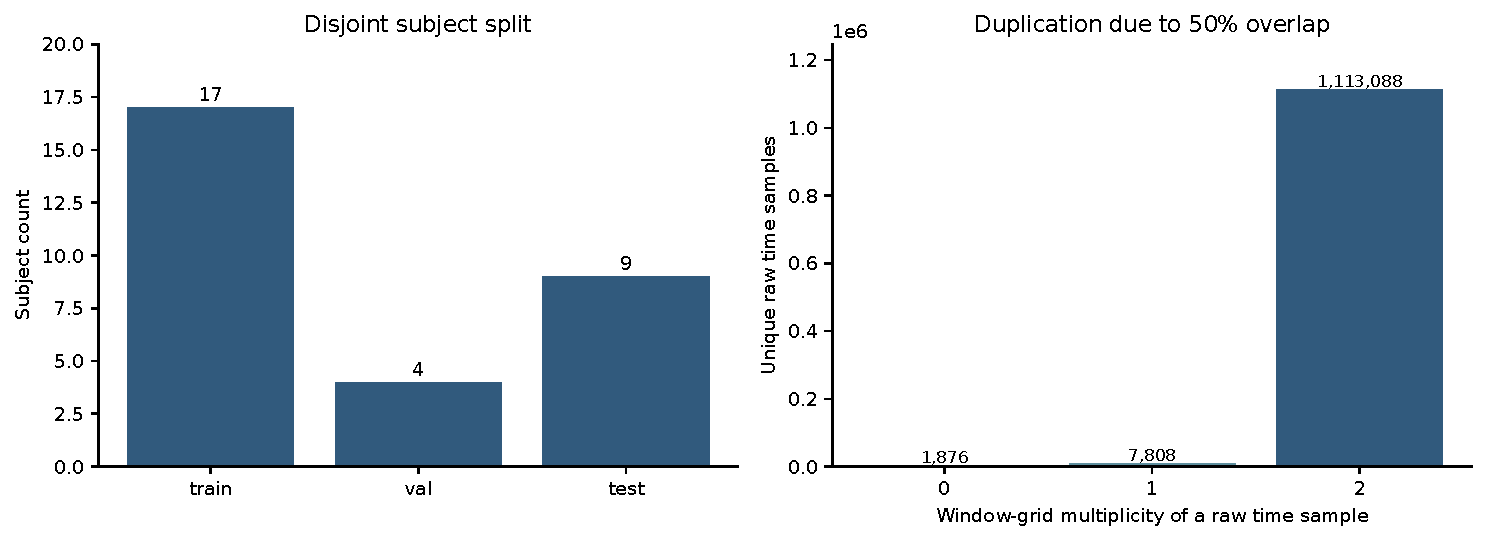
\includegraphics[width=\linewidth]{qa/data_cnn/data_split_multiplicity.pdf}
\caption{Split theo người và số lần mỗi mẫu raw được lưới window sử dụng. Mỗi mẫu chỉ được đếm một lần trong histogram multiplicity.}
\end{figure}

\subsection{Overlap sau căn chỉnh khác khoảng cách cùng tọa độ}
Với hai window kề nhau của cùng recording,
\begin{equation}\label{eq:overlap}
X_{e,k}[:,64:128]=X_{e,k+1}[:,0:64].
\end{equation}
Đây là cùng thời điểm raw được lưu tại hai vị trí tensor khác nhau. Ngược lại,
\begin{equation}\label{eq:delta}
\Delta_{e,k}[c,i]=X_{e,k+1}[c,i]-X_{e,k}[c,i]
=r_e[kS+S+i,c]-r_e[kS+i,c]
\end{equation}
so sánh hai thời điểm cách nhau 1,28 s. Vì thế, equality ở
\eqref{eq:overlap} không buộc $\norm{\Delta}_2$ nhỏ. Phản ví dụ một kênh
$r[n]=n$ cho overlap exact nhưng mỗi tọa độ của $\Delta$ bằng 64. Quy mô
biên độ của ví dụ này chỉ để bác bỏ suy luận logic, không mô phỏng HAPT.

Số cặp kề nhau là $\sum_e(N_e-1)=17453-61=17392$, không phải 17.452:
có 61 điểm bắt đầu recording không được nối qua biên. Mỗi cặp chia sẻ
$6\cdot64=384$ tọa độ, nên kiểm tra exact thực hiện trên
$17392\cdot384=6678528$ giá trị, đều khớp.

\section{Annotation và chính sách nhãn: data sau lọc là gì?}
\subsection{Convention được kế thừa, vấn đề còn mở}
Một dòng annotation có dạng $(e,u,a,b_0,b_1)$: recording, subject, activity,
đầu và cuối span. Source local gán trực tiếp slice Python
\code{labels[start:end+1]}, dùng độ dài inclusive $b_1-b_0+1$; window dùng
slice zero-based có end exclusive. README mô tả chỉ số đầu/cuối nhưng chưa
nói rõ 0-based hay 1-based. Báo cáo giữ convention source để tái tạo số
liệu; việc tái tạo khớp không chứng minh annotation gốc phải được hiểu theo
convention đó. Cần xác minh tài liệu tạo nhãn trước khi đóng băng pipeline mới.

Không tự dịch một mẫu, sửa annotation hoặc nối spans để tạo số liệu đẹp hơn.
Các duration/support bên dưới đều mang điều kiện convention này. Trong
1.122.772 raw samples, 815.614 có annotation theo cách gán hiện hữu, còn
307.158 không có nhãn. Coverage annotation giữa các recording trải từ
39,21281\% đến 80,26243\%. Phần chưa gán không được mặc định là đứng yên,
nhiễu hay một activity thứ 13.

\subsection{Định nghĩa chính xác bốn policy}
Gọi $n_a(X)$ là số trong 128 mẫu được gán activity $a>0$. Tỷ lệ của lớp
chiếm nhiều nhất là
\begin{equation}
p_{\max}(X)=\max_{a\in\{1,\ldots,12\}}\frac{n_a(X)}{128}.
\end{equation}
Mẫu số là toàn window, kể cả mẫu không nhãn. Source chọn
\code{label_majority} bằng lớp có count lớn nhất trong các nhãn dương;
khi đồng hạng, thứ tự của \code{np.unique} và \code{argmax} khiến lớp có ID
nhỏ nhất được chọn. Quy tắc này là metadata convention, không phải quyết
định của CNN.

\begin{tabularx}{\linewidth}{@{}P{2.2cm}Yrr@{}}\toprule
Policy & Điều kiện theo pipeline & Count & Tỷ lệ\\\midrule
pure & Cả 128 mẫu cùng một nhãn dương. & 10.361 & 59,3652\%\\
majority & Không pure; $p_{\max}\ge0,6$. & 1.917 & 10,9838\%\\
ambiguous & Có nhãn dương; $p_{\max}<0,6$. & 1.588 & 9,0987\%\\
unlabeled & Không có nhãn dương; majority ID bằng 0. & 3.587 & 20,5523\%\\\bottomrule
\end{tabularx}

Do count nguyên, ngưỡng 0,6 tương đương tối thiểu
$\lceil0,6\cdot128\rceil=77$ mẫu. Window có 60 mẫu cùng nhãn và 68 mẫu
unlabeled có tỷ lệ $60/128$, không phải $60/60=1$; do đó ambiguous. Một
window chứa 128 mẫu cùng lớp chuyển tư thế vẫn là pure. ``Chuyển tư thế''
là tên lớp, còn ``mixed/ambiguous'' là thuộc tính phân bố nhãn trong window.

Có 1.273 windows có cờ \code{crosses_boundary}, bằng 7,2939\% toàn bộ.
Cờ này của metadata không đồng nghĩa với ambiguous: một window trộn nhiều
nhãn vẫn có thể đạt majority; một window chỉ có một nhãn dương và nhiều
khoảng trống vẫn có thể ambiguous. Không cộng các tỷ lệ ấy như các nhóm rời nhau.

\begin{figure}[htbp]\centering
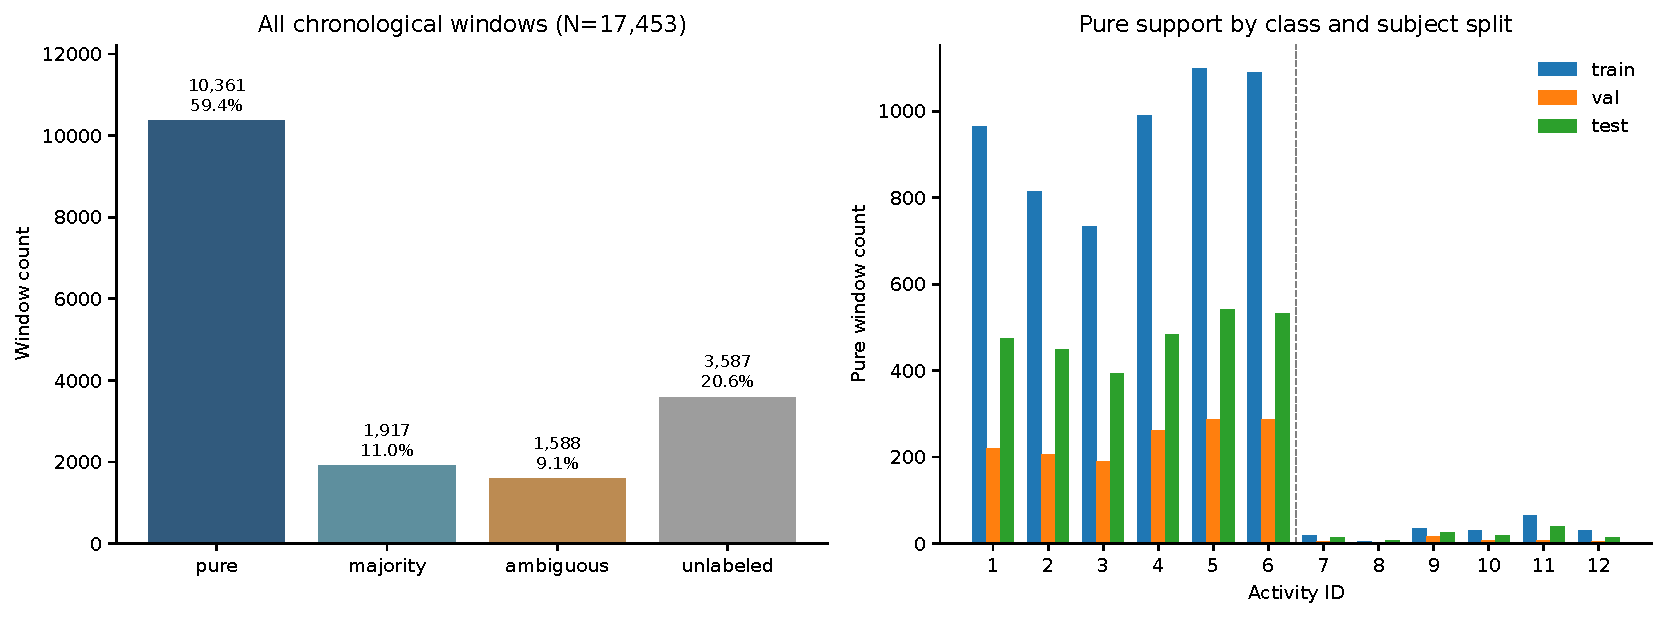
\includegraphics[width=\linewidth]{qa/data_cnn/data_policy_support.pdf}
\caption{Phân bố policy trên toàn stream và pure support theo lớp/split. Vạch giữa ID6 và ID7 tách sáu hoạt động cơ bản khỏi sáu chuyển tư thế.}
\end{figure}

\section{Mười hai lớp, độ dài span và thiên lệch do lưới}
\subsection{Support thực tế sau windowing}
\begin{table}[htbp]\centering\small
\input{qa/data_cnn/data_class_support.tex}
\caption{Pure windows dưới convention hiện hữu. Tổng train/val/test: 5.878/1.490/2.993.}
\end{table}

Pure K12 gồm 10.361 windows, còn pure K6 chỉ giữ ID1--6 và có 10.017.
344 pure windows chuyển tư thế chiếm 3,32014\% pure K12. Chọn K6 vì đã có
checkpoint cũ sẽ thay đổi bài toán và denominator; không xem đó là quyết
định đã được chấp thuận cho nghiên cứu mới. Nếu nghiên cứu mới nhận diện
12 hoạt động, head, class-pair margins, train/test support và protocol đều
phải dùng schema tương ứng.

\subsection{Độ dài hoạt động giải thích mất support thế nào?}
\begin{table}[htbp]\centering
\input{qa/data_cnn/data_class_spans.tex}
\caption{Duration inclusive $(b_1-b_0+1)/50$ của từng annotation span. Không cộng nối qua recording.}
\end{table}

Các span chuyển tư thế có median 2,59--4,73 s, gần thang window 2,56 s;
trong khi span hoạt động cơ bản thường dài hơn rõ rệt. Toàn bộ 358 spans
chuyển tư thế có 67.208 mẫu theo convention inclusive, nhưng việc cắt
pure windows không bảo toàn tỷ lệ duration này. Không suy tỷ lệ raw theo
class trực tiếp từ tỷ lệ pure windows.

\begin{proposition}[Số window thuần nhãn bên trong một span]
Giả sử span inclusive $[a,b]$ nằm trong một recording, có một nhãn, không
chồng lấn, không cần nối với span khác. Lưới window bắt đầu tại $kS$ với
$k\ge0$. Khi $a\ge0$, số window nằm hoàn toàn trong span là
\begin{equation}\label{eq:span}
N_{[a,b]}=\max\left\{0,
\left\lfloor\frac{b-W+1}{S}\right\rfloor
-\left\lceil\frac{a}{S}\right\rceil+1\right\}.
\end{equation}
\end{proposition}
\begin{proof}
Window thuộc span khi và chỉ khi $kS\ge a$ và $kS+W-1\le b$. Suy ra cận
nguyên dưới $\lceil a/S\rceil$ và cận trên $\lfloor(b-W+1)/S\rfloor$.
Đếm số nguyên trong khoảng, lấy 0 nếu cận trên nhỏ hơn cận dưới.
\end{proof}

Điều kiện $b-a+1\ge128$ chỉ là cần, chưa đủ. Ví dụ span $[1,128]$ dài
128: window bắt đầu 0 không thuộc span, window bắt đầu 64 vượt khỏi span,
nên không có pure window. Span $[64,191]$ cũng dài 128 nhưng có một window.
Sự khác biệt là pha của biên annotation đối với lưới stride.

\begin{tabular}{@{}lrrr@{}}\toprule
Nhóm spans & ID1--6 & ID7--12 & Tổng\\\midrule
Ngắn hơn 128 mẫu & 0 & 40 & 40\\
Đủ 128, không có aligned window & 1 & 90 & 91\\
Có ít nhất một aligned window & 855 & 228 & 1.083\\\bottomrule
\end{tabular}

Các số được kiểm độc lập bằng enumerate mọi start $0,64,128,\ldots$ và bằng
\eqref{eq:span}; tổng window nội span là 10.361, khớp pure support. Riêng
SIT\_TO\_STAND có 62 spans: 29 quá ngắn, 21 đủ dài nhưng lệch lưới, chỉ
12 spans còn lại tạo tổng 12 pure windows. Đây là phép giải thích cơ chế
mất quan sát; không khẳng định sửa stride là phương án tối ưu trước khi
xem accuracy, cost, annotation và mục tiêu streaming.

Nếu dùng mixed labels, soft targets, window ngắn hơn hoặc stride khác,
phải ghi đó là phương án nghiên cứu mới và xây dựng lại protocol. Báo cáo
không áp dụng các thay đổi ấy lên dữ liệu nguồn.

\section{Split, phụ thuộc và đơn vị đánh giá}
\subsection{Split hiện hữu được kiểm lại}
\begin{table}[htbp]\centering\small
\begin{tabular}{@{}lrrrrrr@{}}\toprule
Split & Người & Records & Raw samples & All windows & Pure K12 & Pure K6\\\midrule
Train & 17 & 34 & 641.745 & 9.978 & 5.878 & 5.693\\
Validation & 4 & 8 & 155.739 & 2.422 & 1.490 & 1.450\\
Test & 9 & 19 & 325.288 & 5.053 & 2.993 & 2.874\\\bottomrule
\end{tabular}
\caption{Split local theo người; không đồng nhất với một tỷ lệ train/test ghi trên trang dataset.}
\end{table}

Ba tập subject rời nhau; không recording nào bị chia sang nhiều split.
Danh sách người ở Phụ lục~\ref{app:subjects}. Trong mỗi recording,
\code{win_idx} liên tiếp và bắt đầu từ 0. Khi truy cập tensor, phải dùng
global row mapping theo $(exp,win\_idx)$, không dùng riêng \code{win_idx}:
chỉ số này lặp lại giữa các recording. Audit mới merge one-to-one và kiểm
thứ tự global row trước khi lấy dữ liệu.

Số cặp theo split là train 9.944, val 2.414, test 5.034, bằng số windows
trừ số recordings trong từng split. Pure test K6 có 2.874 phần tử chỉ dùng
cho population đã lọc đó; không dùng làm denominator của reuse trên toàn
test stream có 5.053 windows hoặc 5.034 pairs.

\subsection{Vì sao không coi 17.453 windows là i.i.d.?}
Hai windows kề nhau chia sẻ một nửa mẫu. Nhiều recording thuộc cùng người
còn chia sẻ kiểu vận động, vị trí thiết bị và các yếu tố cá nhân. Random
window split có thể đặt cùng raw samples vào train và test. Split theo
người hiện hữu tránh dạng giao nhau đó, nhưng không làm các windows bên
trong một split độc lập.

Với một mean $\bar Z=N^{-1}\sum_iZ_i$, công thức đúng là
\begin{equation}
\operatorname{Var}(\bar Z)=\frac{1}{N^2}
\sum_{i=1}^{N}\sum_{j=1}^{N}\operatorname{Cov}(Z_i,Z_j).
\end{equation}
Rút gọn thành $\sigma^2/N$ cần các covariance ngoài đường chéo bằng 0
và giả thiết variance phù hợp. Tài liệu không ước lượng một ``effective N''
chỉ từ overlap 50\%: quyết định CNN, nhãn và duration có phụ thuộc khác nhau.
Nếu cần uncertainty, một phương án là resample theo subject/recording và
giữ trật tự bên trong; cần báo rõ design và số cluster, nhất là val chỉ có
bốn người. Đó là thiết kế đề xuất, chưa phải kết quả bootstrap đã chạy.

\subsection{Vai trò test trong một tài liệu exploratory}
Các bảng mô tả và ECDF ở đây xem cả ba splits để hiểu snapshot. Do đó, chúng
không đóng vai trò một lần xác nhận held-out chưa từng được quan sát. Nếu
chọn thresholds hoặc kiến trúc từ các hình all-split này, cần ghi nhận việc
đó và có giao thức xác nhận độc lập về sau. Việc chuẩn hóa chỉ fit train
không tự biến mọi phân tích tiếp theo thành một đánh giá blind.

\section{Phân bố channel, scale và normalization}
\subsection{Thống kê trên raw samples duy nhất}
\begin{table}[htbp]\centering\scriptsize
\resizebox{\linewidth}{!}{\input{qa/data_cnn/data_channel_statistics.tex}}
\caption{Thống kê trên 1.122.772 raw rows duy nhất, đọc từ text sang float64; std dân số (ddof=0). Không đếm lặp overlap.}
\end{table}

Mean acc\_x xấp xỉ 0,81933 g, khác xa zero; đây là tín hiệu rằng orientation
và thành phần trọng lực cần được hiểu trước khi đặt budget. Các quantile
cho thấy cả sáu kênh có thang và đuôi khác nhau. Những nhận xét này là mô
tả giá trị và giải thích khả dĩ; chưa xác định nguyên nhân vật lý của mỗi
outlier. Báo cáo không cắt bỏ các cực trị hoặc gọi chúng là lỗi đo.

Mean/std trong bảng được tính trên raw duy nhất toàn bộ splits để mô tả
snapshot. Chúng không được dùng fit preprocessing của một classifier.
Tổng hợp nhiều người bằng pooled rows còn khiến người có recording dài
đóng góp nhiều hơn; nếu cần đặc trưng của ``người trung bình'', cần báo thêm
thống kê cân bằng theo subject. Hai estimand này không giống nhau.

\begin{figure}[htbp]\centering
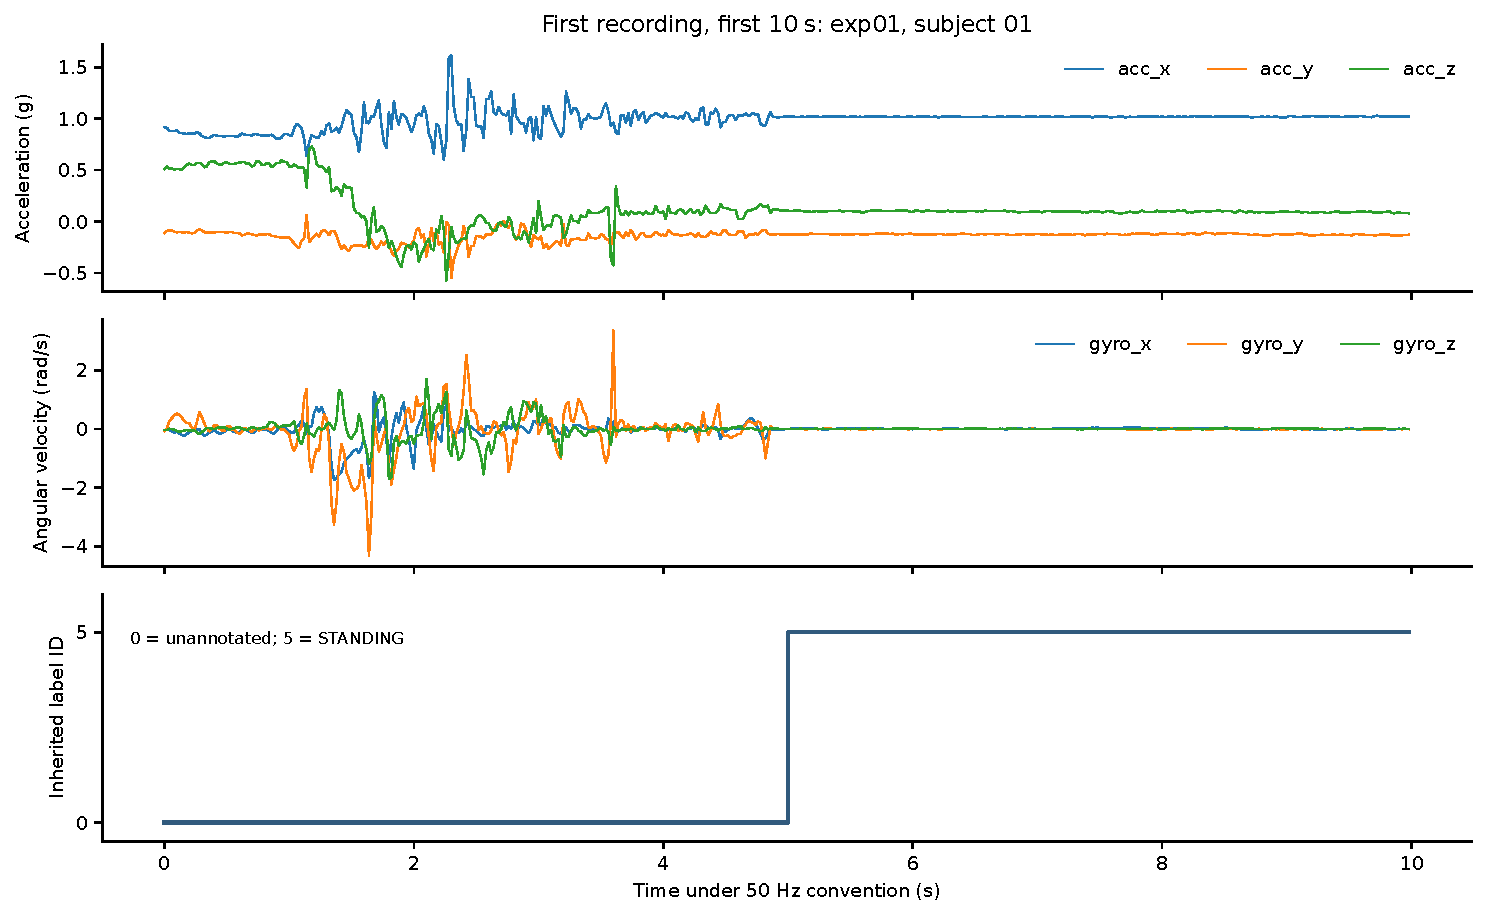
\includegraphics[width=0.98\linewidth]{qa/data_cnn/data_raw_first_recording.pdf}
\caption{Mười giây đầu của recording đầu tiên theo thứ tự tên tệp: exp01, subject01. Chọn xác định để minh họa cách đọc sáu kênh và label0/5; không chọn theo hiệu quả model hay độ đẹp của waveform.}
\end{figure}

\subsection{Normalizer cố định được dùng trong audit khoảng cách}
Để cung cấp khoảng cách dimensionless trong một hệ tọa độ tái lập được,
audit dùng đúng convention mean/std \code{float32} của source cũ: fit trên
5.693 pure K6 train windows, gộp axes $(0,2)$, clip std tối thiểu $10^{-6}$.
Đây là một lựa chọn phân tích kế thừa được khai báo, không phải pipeline
cuối cùng của mô hình K12 mới.
\begin{equation}
Z[c,i]=\frac{X[c,i]-\mu_c}{\sigma_c},\quad
\mu_c=\frac{1}{128N_{tr}}\sum_{w\in tr}\sum_i X_w[c,i].
\end{equation}
Std dùng cùng population được fit, ddof=0. Các tham số cố định:
\begin{center}\begin{tabular}{@{}lrr@{}}\toprule
Channel & $\mu_c$ & $\sigma_c$\\\midrule
acc\_x & 0,804849 & 0,413195\\
acc\_y & 0,030074 & 0,402293\\
acc\_z & 0,080927 & 0,356522\\
gyro\_x & 0,004974 & 0,417901\\
gyro\_y & $-0,002906$ & 0,406792\\
gyro\_z & $-0,007806$ & 0,261610\\\bottomrule
\end{tabular}\end{center}

Vì fit trên overlapping windows, raw sample được cân theo số lần xuất hiện
trong tập pure đã lọc. Do đó, các số này không nhất thiết bằng mean/std
raw duy nhất chỉ của train. Nó cũng loại bỏ các lớp chuyển tư thế khỏi fit.
Nếu nghiên cứu mới dùng K12 hoặc all-stream training, cần chọn và đóng băng
fit population phù hợp trước đánh giá; không lấy bảng toàn dataset để thay
âm thầm các tham số này.

\subsection{Normalization thay đổi hình học của miền}
Với $D$ là ma trận chéo lặp $\sigma_c$ cho 128 vị trí của mỗi channel,
\begin{equation}
\Delta z=D^{-1}\Delta x,\quad
\norm{\Delta z}_2^2=\sum_{c,i}\frac{\Delta x[c,i]^2}{\sigma_c^2}.
\end{equation}
Khoảng cách raw cộng bình phương g với rad/s không có một đơn vị vật lý
chung. Nó vẫn là đại lượng số tái lập được nhưng phụ thuộc cách biểu diễn
đơn vị. Khoảng cách normalized dimensionless khắc phục sự trộn đơn vị trực
tiếp, song vẫn phụ thuộc fit population; không trở thành chứng nhận invariant.

Nếu miền raw là $|\Delta x_i|\le b_i$, miền normalized đúng là
$|\Delta z_i|\le b_i/\sigma_i$ khi $\sigma_i>0$. Ngược lại budget
normalized $\beta_i$ tương ứng raw $b_i=\sigma_i\beta_i$. Phải cùng một
hệ tọa độ ở lúc fit miền, membership và bound reference $F=f_\theta\circ N$.
Nếu normalize riêng mỗi window, $N$ không còn là ánh xạ affine cố định ấy;
các đẳng thức và bounds phải được xét lại.

\section{Tính liên tục thời gian: bốn loại correlation}
\subsection{Định nghĩa đối tượng trước khi đọc hệ số}
Pearson correlation giữa vectors $a,b$ dài $m$ là
\begin{equation}
\operatorname{corr}(a,b)=\frac{\sum_i(a_i-\bar a)(b_i-\bar b)}
{\sqrt{\sum_i(a_i-\bar a)^2\sum_i(b_i-\bar b)^2}},
\end{equation}
khi hai variance đều dương. Correlation gần 1 thể hiện quan hệ tuyến tính
sau centering, không buộc $a=b$; ví dụ $b=10a+100$ vẫn cho 1. Bốn phép đo:
\begin{enumerate}
\item \textbf{Raw lag1}: corr giữa $r_e[0:T_e-1,c]$ và $r_e[1:T_e,c]$;
độ trễ danh định 20 ms.
\item \textbf{Raw lag64}: corr giữa $r_e[0:T_e-64,c]$ và
$r_e[64:T_e,c]$; độ trễ 1,28 s.
\item \textbf{Window positional}: corr của hai vectors 128 vị trí cùng
channel trong hai windows kề nhau, chưa dịch chỉ số. Tính từng pair rồi
mean trong recording, sau đó mean qua recordings.
\item \textbf{Window channel-mean}: đặt $g_k=128^{-1}\sum_iX_{e,k}[c,i]$,
tính corr giữa chuỗi $g_0,\ldots,g_{N_e-2}$ và $g_1,\ldots,g_{N_e-1}$.
\end{enumerate}
Ba loại còn lại cũng tính riêng từng recording rồi lấy arithmetic mean
61 recordings. Đó là mean của các correlation, không phải correlation của
một vector được nối qua biên recording; recording dài/ngắn nhận cùng trọng
số ở bước mean cuối. Bảng không ước lượng population correlation với CI.

\begin{table}[htbp]\centering\small
\begin{tabular}{@{}lrrrr@{}}\toprule
Channel & Raw lag1 & Raw lag64 & Positional & Channel-mean\\\midrule
acc\_x & 0,9716 & 0,7209 & 0,0119 & 0,9661\\
acc\_y & 0,9778 & 0,8240 & 0,0224 & 0,9717\\
acc\_z & 0,9773 & 0,7769 & 0,0485 & 0,9360\\
gyro\_x & 0,9550 & 0,1484 & $-0,0307$ & 0,6614\\
gyro\_y & 0,8297 & 0,0606 & $-0,0137$ & 0,5596\\
gyro\_z & 0,9183 & 0,0960 & $-0,0095$ & 0,6134\\\bottomrule
\end{tabular}
\caption{Tính mới trực tiếp trên raw rows và window pairs đúng recording; định nghĩa và aggregation như mô tả.}
\end{table}

\subsection{Giải thích kết quả và một sai khác nguồn cần giữ rõ}
Raw lag1 cao phù hợp với thay đổi nhỏ trong 20 ms. Ở lag64, các trục gyro
có correlation thấp hơn nhiều; quan hệ 20 ms không được ngoại suy sang
query stride 1,28 s. Positional correlation gần zero không mâu thuẫn với
overlap exact: nó so sánh các vị trí khác thời gian theo \eqref{eq:delta}.
Channel means ổn định hơn shape của toàn window; đó là động cơ xem xét
summary/structured domains, chưa chứng minh summary ấy đủ quyết định lớp.

Audit phát hiện \code{scripts/06b_corr_semantics.py} tạo ``raw series'' bằng
\code{ravel()} trên các overlapping windows. Phép nối này lặp mẫu và tạo
các bước nhảy nhân tạo tại biên window, nên không cùng định nghĩa với raw
lag1/lag64 trực tiếp ở trên. Các số cũ trong \code{data/corr_semantics.json}
không được dùng thay cho bảng này. Báo cáo mới chỉ đọc và ghi rõ khác biệt,
không sửa source/artifact cũ. Điều này minh họa vì sao cần kiểm đối tượng
được correlate trước khi suy luận tính chất data.

\section{Khoảng cách giữa windows: phân tầng thay cho một con số}
\subsection{Ba nhóm pairs rời nhau}
Audit chia toàn bộ 17.392 adjacent pairs thành:
\begin{equation*}
\begin{array}{lr}
\text{Cả hai pure, cùng label\_majority:}&9.278,\\
\text{label\_majority khác nhau:}&1.651,\\
\text{Cùng majority ID nhưng không cùng pure:}&6.463.
\end{array}
\end{equation*}
Nhóm thứ ba bao gồm equal nonpure và cả unlabeled ID0. Nhóm ``change'' có
thể đi từ/đến ID0 hoặc mixed window; không đồng nghĩa một chuyển tư thế
ground truth đã được xác minh, cũng không phải thay đổi prediction. Hai
nhóm đầu rời nhau nhưng không phủ toàn bộ pair population. Không bỏ nhóm
thứ ba khỏi mẫu số all-stream coverage mà không nêu rõ.

Đặt $d_2=\norm{\operatorname{vec}(Z_{k+1}-Z_k)}_2$ và
$d_\infty=\max_{c,i}|Z_{k+1}[c,i]-Z_k[c,i]|$. Dùng cùng-coordinate delta,
không phải overlap difference sau căn chỉnh. Với 768 tọa độ,
\begin{equation}
d_\infty\le d_2\le\sqrt{768}\,d_\infty.
\end{equation}
Những cận này chỉ liên hệ hai norm của một vector; không chuyển quantile
của một norm thành quantile chính xác của norm còn lại.

\begin{table}[htbp]\centering\small
\begin{tabular}{@{}llrrr@{}}\toprule
Hệ tọa độ & Nhóm / norm & p50 & p90 & p99\\\midrule
Raw, trộn units & Same-pure / $L_2$ & 1,84282 & 17,35410 & 24,18713\\
Raw, trộn units & Majority-change / $L_2$ & 13,26583 & 22,97948 & 29,56845\\
Normalized & Same-pure / $L_2$ & 4,93575 & 46,41709 & 65,26317\\
Normalized & Majority-change / $L_2$ & 36,56520 & 59,33480 & 77,60553\\
Normalized & Same-pure / $L_\infty$ & 0,98734 & 7,06383 & 12,31258\\
Normalized & Majority-change / $L_\infty$ & 5,81409 & 9,47326 & 15,07550\\\bottomrule
\end{tabular}
\caption{Quantiles pooled mô tả toàn snapshot, không phải threshold được fit/test cho một classifier.}
\end{table}

\begin{figure}[htbp]\centering
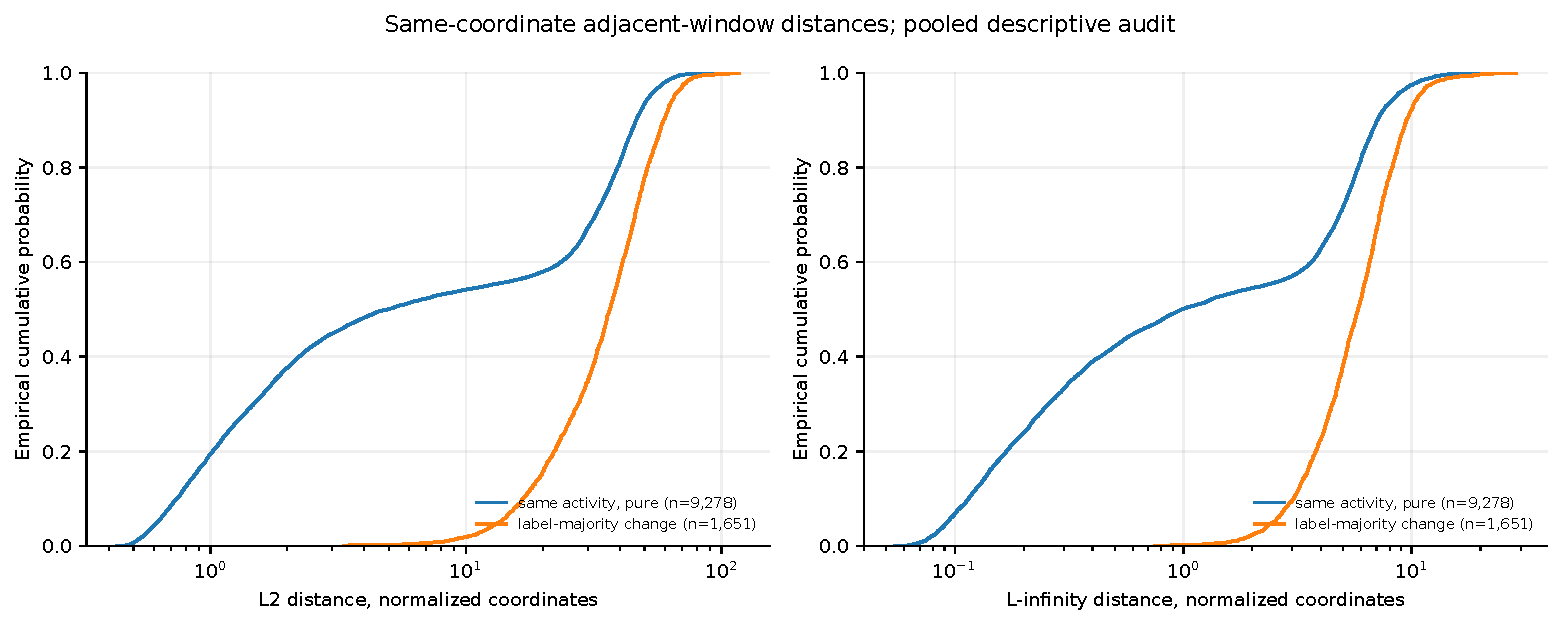
\includegraphics[width=\linewidth]{qa/data_cnn/data_normalized_distances.pdf}
\caption{Empirical CDF của hai nhóm, trục khoảng cách logarithmic. Normalizer fit pure K6 train và cố định cho mọi split. Hai phân bố chồng lấn; không có ranh giới quyết định CNN nào được đo trong hình.}
\end{figure}

Median same-pure nhỏ hơn change nhưng đuôi same-pure lớn và có overlap.
Không thể lấy một percentile rồi kết luận mọi pair dưới ngưỡng chắc chắn
cùng prediction. ``Same activity'' là ground-truth metadata; một reference
classifier có thể sai hoặc nhạy với pha dù nhãn không đổi.

\subsection{Theo lớp: vì sao pooled median che khuất cấu trúc?}
\begin{table}[htbp]\centering\small
\begin{tabular}{@{}lrrr@{}}\toprule
Activity ID & Same-pure pairs & Median normalized $L_2$ & p90 normalized $L_2$\\\midrule
1 & 1.534 & 36,43503 & 49,93195\\
2 & 1.285 & 32,85961 & 47,99001\\
3 & 1.131 & 44,86683 & 60,33992\\
4 & 1.616 & 1,08972 & 3,62727\\
5 & 1.806 & 1,75657 & 7,56076\\
6 & 1.790 & 1,35659 & 3,95880\\
7 & 8 & 45,95473 & 57,19978\\
8 & 0 & không xác định & không xác định\\
9 & 27 & 45,08910 & 53,99518\\
10 & 13 & 41,32653 & 49,87594\\
11 & 57 & 39,92019 & 51,32326\\
12 & 11 & 39,97517 & 49,35115\\\bottomrule
\end{tabular}
\caption{Cùng activity không tạo một thang khoảng cách đồng nhất. Quantiles nhóm ít mẫu chỉ là thống kê finite-sample, không được trình bày như ước lượng ổn định.}
\end{table}

Các lớp đi lại 1--3 có median lớn hơn các tư thế tĩnh 4--6. Điều này phù
hợp với khả năng shape thay đổi theo pha chuyển động. Chưa kiểm định một
mô hình periodic hoặc causal nào, nên không gán mọi chênh lệch cho pha.
Lớp8 có support pure nhưng không có same-pure adjacent pair; không được
điền distance zero hoặc bỏ tên lớp khỏi bảng để tránh ô trống.

Về thiết kế đánh giá, nên báo coverage/fallback theo lớp và policy bên cạnh
tổng all-stream, đồng thời tách nhãn thật dùng cho hậu kiểm khỏi tín hiệu
có thể biết lúc chạy. Một event selector runtime không được truy cập
ground-truth activity của window hiện tại chỉ vì audit chia nhóm theo nhãn.

\section{Từ đặc điểm data đến miền ECDR và nghĩa vụ chứng minh}
\subsection{Quan hệ trực tiếp với bài toán}
Gọi $N$ là normalization cố định, $f_\theta$ trả vector logits và
$F=f_\theta\circ N$. Với anchor $X^r$ đã chạy reference, đặt
$c=\arg\max_jF_j(X^r)$. Một miền $\mathcal S_e(X^r)$ có thể được đề xuất
từ train data và trạng thái quan sát được. Điều kiện để tái dùng nhãn $c$ là
\begin{equation}\label{eq:cert}
X_t\in\mathcal S_e(X^r),\qquad
\underline m_{cj}(\mathcal S_e)>0\quad\text{với mọi }j\ne c,
\end{equation}
trong đó mỗi $\underline m_{cj}$ là lower bound sound của
$\inf_{X\in\mathcal S_e}[F_c(X)-F_j(X)]$. Data giúp định nghĩa và đánh giá
membership của miền; classifier/verifier mới quyết định margin có dương
trên toàn miền hay không. Tính đúng của implication dùng mọi điểm trong
miền, không chỉ các pairs trong dataset.

\begin{tabularx}{\linewidth}{@{}P{3.1cm}Y Y@{}}\toprule
Quan sát data & Hướng xây dựng có cơ sở & Điều còn phải chứng minh/đo\\\midrule
Overlap exact sau dịch & Miền shift-plus-tail, hoặc structured wave domain. & Bound trên tail/residual; xử lý biên CNN và certificate của quyết định.\\
Scale khác theo channel & Budget diagonal trong hệ tọa độ cố định. & Membership đúng normalization; class-pair bounds đủ chặt.\\
Distance khác theo hoạt động & Nhiều budget/template theo tín hiệu runtime. & Không dùng nhãn thật lúc chạy; selector cost và coverage xác nhận riêng.\\
Summary ổn định hơn shape & Miền có phần summary và residual có cận. & Mọi residual hợp lệ đều được bound; không chỉ reconstruction error trung bình.\\
Transition support thấp & Báo cáo riêng mixed/transitions và per-class. & Reference đủ tin cậy; không có evidence mất đi do chỉ chọn pure K6.\\\bottomrule
\end{tabularx}

\subsection{Vì sao quantile không phải chứng nhận joint?}
Ví dụ fit $b_i$ là q90 của $|\Delta z_i|$ trên train pairs. Điều này cho
một budget mô tả theo từng tọa độ. Membership box cần \emph{đồng thời}
$|\Delta z_i|\le b_i$ cho cả 768 tọa độ. Marginal 90\% không suy ra joint
90\%. Nếu độc lập lý tưởng và đúng xác suất 0,9 từng tọa độ, joint là
$0,9^{768}\approx7,22\cdot10^{-36}$; giả thiết độc lập này không được áp
cho HAPT, chỉ minh họa sự khác nhau giữa hai câu hỏi. Union bound
$P(\exists i\text{ vượt})\le\sum_iP(i\text{ vượt})$ cũng có thể cho cận
vô ích nếu tổng lớn hơn 1.

Ngay cả khi đo được empirical joint membership cao, nó vẫn chỉ đo tần suất
pairs trong tập đã quan sát nằm trong miền; chưa chứng minh
\eqref{eq:cert}. Một miền quá rộng có thể chứa nhiều data nhưng không thể
chứng nhận. Một miền rất nhỏ có thể dễ chứng nhận nhưng coverage thấp.
Cần phân tích hai trục và total runtime cost cùng lúc.

\subsection{Wave domain: giữ structure mà không lược bỏ nhiễu}
Trong hệ tọa độ normalized, một biểu diễn lý thuyết là
\begin{equation}
z_t=T_Sz^r+Vu+r,\qquad u\in\mathcal U,\quad r\in\mathcal R.
\end{equation}
$T_S$ là phép dịch/copy phần overlap cùng convention padding/tail được
định nghĩa; $Vu$ biểu diễn thay đổi có cấu trúc, $r$ chứa phần chưa giải
thích. Không lấy $T_Sz^r$ như toàn window thực nếu tail chưa được xác định.
Nếu $V$ học bằng PCA, variance explained là average reconstruction
criterion; không có nghĩa $r=0$ hoặc mọi query tương lai đều có residual
nhỏ. Cần cận residual và membership trước khi áp certificate.

Một minh họa pha: $s[n]=A\sin(\omega n+\phi)$ cho
\begin{equation}
s[n+S]-s[n]=2A\sin(\omega S/2)
\cos(\omega n+\phi+\omega S/2).
\end{equation}
Cùng một chuyển động periodic có thể tạo same-coordinate delta lớn khi
$\omega S/2$ gần $\pi/2$, dù overlap sau căn chỉnh vẫn exact. Ví dụ giải
thích tại sao kiến trúc/miền cần quan tâm dịch thời gian; không fit hay xác
nhận mô hình sinusoid trên HAPT bằng công thức này.

\subsection{Một bước kề nhau không bảo đảm anchor sống nhiều bước}
Phân bố $X_{t+1}-X_t$ mô tả adjacent pairs, còn reuse từ anchor $X^r$ tại
nhiều thời điểm cần membership $X_t\in\mathcal S(X^r)$. Hai đại lượng không
thể thay thế. Từ triangle inequality,
\begin{equation}
\norm{X_t-X^r}\le\sum_{i=r}^{t-1}\norm{X_{i+1}-X_i},
\end{equation}
nên nhiều bước nhỏ vẫn có thể tích lũy thành drift lớn. Không tự di chuyển
tâm certificate sang query vừa hit nếu chưa có chứng nhận tại tâm mới.
Muốn đo lifetime phải replay theo recording, giữ anchor/state đúng giao
thức và ghi lại thời điểm refresh; audit adjacent ở đây chưa đo lifetime.

\section{Thiết kế đánh giá được dữ liệu này yêu cầu}
\subsection{Phân biệt đúng các loại kết quả}
Reference classification đánh giá đúng/sai so với nhãn trên population
được định nghĩa. Decision reuse agreement đánh giá nhãn reuse bằng nhãn
reference cho cùng query. Sound certification yêu cầu implication trên
toàn miền đúng với numerical semantics đã chọn. Runtime benefit so tổng
chi phí hệ thống. Bốn mục tiêu liên quan nhưng không tương đương.

Khi reference sai nhãn thật, reuse đúng reference vẫn có thể sai nhãn thật.
Ngược lại, accuracy cao trên pure test không chứng minh an toàn reuse trên
mixed stream. Vì vậy phải cùng báo accuracy của reference, certified
coverage và agreement/runtime trên các denominator tương ứng.

\begin{tabularx}{\linewidth}{@{}P{3cm}Y Y@{}}\toprule
Đại lượng & Mẫu số cần nêu & Trạng thái tài liệu\\\midrule
Pure K12 accuracy & 2.993 pure test windows nếu giữ split hiện tại. & Chưa chạy một CNN K12 mới.\\
All-stream membership & 5.053 test queries, hoặc 5.034 adjacent pairs nếu đúng protocol pairwise. & Chưa chọn/finalize miền mới.\\
Per-class coverage & Queries thuộc lớp/policy được định nghĩa, kể cả trường hợp zero support. & Đã có support mô tả; chưa certified coverage.\\
Multi-step reuse & Queries replay theo recording với anchor lifecycle. & Chưa replay một verifier mới.\\
Net saving & Tổng thời gian/energy gồm selector, membership, build, refresh và fallback. & Không benchmark trong audit này.\\\bottomrule
\end{tabularx}

Nếu build rate là $q$ trên mỗi query và certified reuse rate là $r$, một
cost model đơn giản là
\begin{equation}
\mathbb E[T]\approx T_e+T_m+(1-r)T_f+qT_b.
\end{equation}
Hòa vốn đòi hỏi $rT_f>T_e+T_m+qT_b$. Data hiện cho quy mô input, query
stride và các strata; chưa cho $T_b,T_m,r$ của phương pháp mới. Không đưa
latency checkpoint cũ vào đây như phép đo CNN valid/GAP hay toàn pipeline mới.

\subsection{Các lựa chọn phải đóng băng trước xác nhận mới}
Các quyết định còn mở gồm schema K12 hay task subset có lý do; xử lý
mixed/unlabeled; convention annotation đã xác minh; train-fit population
cho normalizer; window/stride; reference architecture và numerical mode;
domain family; lifecycle/refresh; metric và denominator. Cần ghi các lựa
chọn này trong protocol, rồi chọn miền trên train/validation phù hợp và
đánh giá với một kế hoạch xác nhận được công bố rõ. Báo cáo không tự thay
đổi chúng chỉ để đồng bộ với checkpoint cũ.

\section{Kết quả đã có, giả thuyết còn mở và cách tái lập}
\subsection{Evidence ledger}
\begin{longtable}{@{}P{1cm}P{6.0cm}P{5.7cm}@{}}\toprule
ID & Phát biểu & Trạng thái và evidence\\\midrule\endhead
D01 & Tensor tái tạo từ raw dưới cùng phép cắt/ép kiểu. & VERIFIED bằng toàn bộ 13.403.904 tọa độ, 0 mismatch.\\
D02 & Aligned overlap bằng nhau cho mọi pair kề cùng recording. & VERIFIED 17.392 pairs; có chứng minh từ định nghĩa window.\\
D03 & Các splits không chia sẻ subject/recording. & VERIFIED bằng metadata và tập người; không là bằng chứng i.i.d.\\
D04 & Pure policy làm giảm mạnh transition support. & VERIFIED counts, span lengths và brute-force grid enumeration.\\
D05 & Raw lag1 cao nhưng same-coordinate delta có thể lớn. & VERIFIED thống kê mô tả trên snapshot; không ngoại suy universal.\\
D06 & Annotation indexing hiện hữu đúng ngữ nghĩa gốc. & OPEN; tái tạo source không giải quyết tài liệu 0/1-based.\\
D07 & Miền có cấu trúc tăng certified reuse hữu ích. & HYPOTHESIS; chưa có verifier/model mới và đánh giá matched.\\
D08 & Decision reuse tạo net saving. & HYPOTHESIS; cần total cost và replay đúng lifecycle.\\
D09 & Reference mới giữ được 12 lớp với chất lượng phù hợp. & OPEN; không suy từ checkpoint K6 hay metadata support.\\\bottomrule
\end{longtable}

\subsection{Lệnh tái lập và trách nhiệm artifact}
Từ repository root:
\begin{quote}\small\ttfamily
.venv/bin/python me/qa/data\_cnn/prepare\_data\_analysis.py
\end{quote}
Script chỉ đọc raw, NPZ, Parquet, label names và source/config liên quan;
ghi JSON, bảng và bốn figure PDF/PNG vào \code{me/qa/data_cnn}. Cần NumPy,
Pandas với Parquet backend và Matplotlib. Script không fit CNN, chạy
checkpoint, benchmark, sửa annotation hay thay split. Hash nguồn và kết
quả per-record nằm trong JSON để kiểm tra drift giữa các lần chạy.

Biên dịch tài liệu này bằng Tectonic từ source được lưu, giữ nguyên thư
mục \code{qa/data_cnn} vì figures và tables là companion assets. Kết quả
PDF được kiểm văn bản, references/citations và render để kiểm bố cục;
kiểm artifact không phải một formal proof checker cho verifier ECDR.

\appendix
\clearpage
\section{Danh sách người và raw recordings}\label{app:subjects}
Train gồm subjects 1,3,5,6,7,8,11,14,15,16,17,19,21,22,23,25,26.
Validation gồm 27,28,29,30. Test gồm 2,4,9,10,12,13,18,20,24.
Độ dài $T$ trong bảng là số raw rows của một recording; duration sample-count
là $T/50$. Danh sách đầy đủ giúp đối chiếu tổng và tránh gộp các recordings
cùng người thành một timeline.

\input{qa/data_cnn/data_recording_inventory.tex}

\section{Bản đồ nguồn để đọc tiếp}
\begin{tabularx}{\linewidth}{@{}P{4.0cm}Y@{}}\toprule
Nguồn & Nội dung đối chiếu\\\midrule
\code{ECDR_Weeks_1_2_3_Theory.tex} & Project brief, hệ ký hiệu chuẩn, giả thuyết Week1--3 và điều kiện chứng nhận.\\
\code{ECDR_Mathematics_Explained.tex} & Giải từng bước phép suy ra, các loại cận, support function và lifecycle.\\
\code{ECDR_CNN_Model_Analysis.tex} & Bóc tách CNN valid/ReLU/GAP, kích thước, chi phí và cầu nối tới margins.\\
\code{scripts/03_build_windows.py} & Phép cắt raw và gán label policy được audit tái tạo.\\
\code{scripts/backbone.py} & Convention normalization kế thừa dùng riêng cho audit khoảng cách này.\\
\code{qa/data_cnn/data_analysis.json} & Số liệu mới, hash, conventions và các giới hạn đã khai báo.\\\bottomrule
\end{tabularx}

\begin{thebibliography}{9}
\bibitem{uci} J.-L. Reyes-Ortiz et al. \emph{Smartphone-Based Recognition of
Human Activities and Postural Transitions}. UCI Machine Learning Repository,
dataset 341. Metadata truy cập ngày 28/10/2026.
\url{https://archive.ics.uci.edu/dataset/341/smartphone+based+recognition+of+human+activities+and+postural+transitions}.
\bibitem{local} ECDR workspace. \emph{RawData, window artifacts và fresh
read-only audit}. Các tệp local được liệt kê kèm SHA256 trong
\code{qa/data_cnn/data_analysis.json}; phép tính bởi
\code{qa/data_cnn/prepare_data_analysis.py}, 28/10/2026. Đây là evidence
local, không phải nguồn thực nghiệm được bình duyệt.
\end{thebibliography}
\end{document}
